\begin{figure}
    \centering
    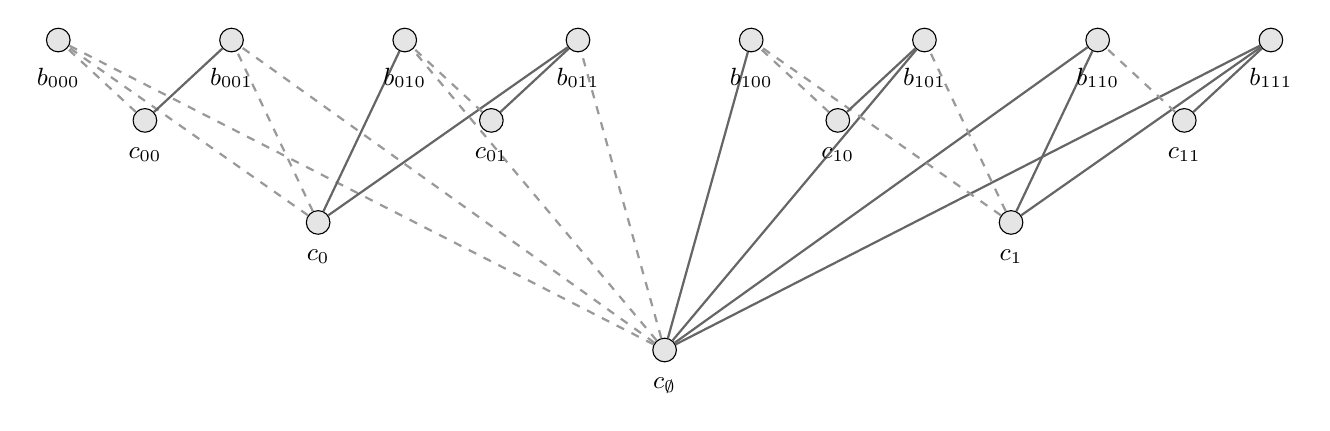
\begin{tikzpicture}[
        vertex/.style={circle, draw, fill=gray!20, minimum size=0.3cm, inner sep=1pt},
        label/.style={below=2pt, font=\small},
        solid edge/.style={draw, thick, black!60},
        dashed edge/.style={draw, dashed, thick, black!40},
    ]
	\node[vertex] (c_) at (8.8,0.0) {};
	\node[vertex] (c_0) at (4.4,1.62) {};
	\node[vertex] (c_1) at (13.200000000000001,1.62) {};
	\node[vertex] (c_00) at (2.2,2.9160000000000004) {};
	\node[vertex] (c_01) at (6.6000000000000005,2.9160000000000004) {};
	\node[vertex] (c_10) at (11.0,2.9160000000000004) {};
	\node[vertex] (c_11) at (15.400000000000002,2.9160000000000004) {};
	\node[vertex] (b_000) at (1.1,3.9366000000000008) {};
	\node[vertex] (b_001) at (3.3000000000000003,3.9366000000000008) {};
	\node[vertex] (b_010) at (5.5,3.9366000000000008) {};
	\node[vertex] (b_011) at (7.700000000000001,3.9366000000000008) {};
	\node[vertex] (b_100) at (9.9,3.9366000000000008) {};
	\node[vertex] (b_101) at (12.100000000000001,3.9366000000000008) {};
	\node[vertex] (b_110) at (14.3,3.9366000000000008) {};
	\node[vertex] (b_111) at (16.5,3.9366000000000008) {};
	\draw[dashed edge] (c_) -- (b_000);
	\draw[dashed edge] (c_) -- (b_001);
	\draw[dashed edge] (c_) -- (b_010);
	\draw[dashed edge] (c_) -- (b_011);
	\draw[solid edge] (c_) -- (b_100);
	\draw[solid edge] (c_) -- (b_101);
	\draw[solid edge] (c_) -- (b_110);
	\draw[solid edge] (c_) -- (b_111);
	\draw[dashed edge] (c_0) -- (b_000);
	\draw[dashed edge] (c_0) -- (b_001);
	\draw[solid edge] (c_0) -- (b_010);
	\draw[solid edge] (c_0) -- (b_011);
	\draw[dashed edge] (c_1) -- (b_100);
	\draw[dashed edge] (c_1) -- (b_101);
	\draw[solid edge] (c_1) -- (b_110);
	\draw[solid edge] (c_1) -- (b_111);
	\draw[dashed edge] (c_00) -- (b_000);
	\draw[solid edge] (c_00) -- (b_001);
	\draw[dashed edge] (c_01) -- (b_010);
	\draw[solid edge] (c_01) -- (b_011);
	\draw[dashed edge] (c_10) -- (b_100);
	\draw[solid edge] (c_10) -- (b_101);
	\draw[dashed edge] (c_11) -- (b_110);
	\draw[solid edge] (c_11) -- (b_111);
	\node[label] at (c_.south) {$c_{\emptyset}$};
	\node[label] at (c_0.south) {$c_{0}$};
	\node[label] at (c_1.south) {$c_{1}$};
	\node[label] at (c_00.south) {$c_{00}$};
	\node[label] at (c_01.south) {$c_{01}$};
	\node[label] at (c_10.south) {$c_{10}$};
	\node[label] at (c_11.south) {$c_{11}$};
	\node[label] at (b_000.south) {$b_{000}$};
	\node[label] at (b_001.south) {$b_{001}$};
	\node[label] at (b_010.south) {$b_{010}$};
	\node[label] at (b_011.south) {$b_{011}$};
	\node[label] at (b_100.south) {$b_{100}$};
	\node[label] at (b_101.south) {$b_{101}$};
	\node[label] at (b_110.south) {$b_{110}$};
	\node[label] at (b_111.south) {$b_{111}$};
    \end{tikzpicture}
    \caption{Example of a 3-tree. 
Notice that connections between disjoint sub-trees are not defined, and may be edges or non-edges in 
any combination.}
    \label{fig:k_tree}
\end{figure}
